\documentclass{article}
\usepackage{tikz}
\usepackage{amsmath} % For math symbols like \mathcal, \theta
\usepackage{xcolor}
\usetikzlibrary{
    patterns,
    positioning,    % For relative node placement (right=of, etc.)
    arrows.meta,    % For arrow tip styles like Stealth
    shapes.geometric,% For shapes like rectangle and trapezium
    calc            % For coordinate calculations ($(...)!,! (...)$)
}

% Define a light blue color for the network fill
\definecolor{lightblue}{RGB}{210, 225, 240}

\begin{document}

\begin{figure}[htbp]
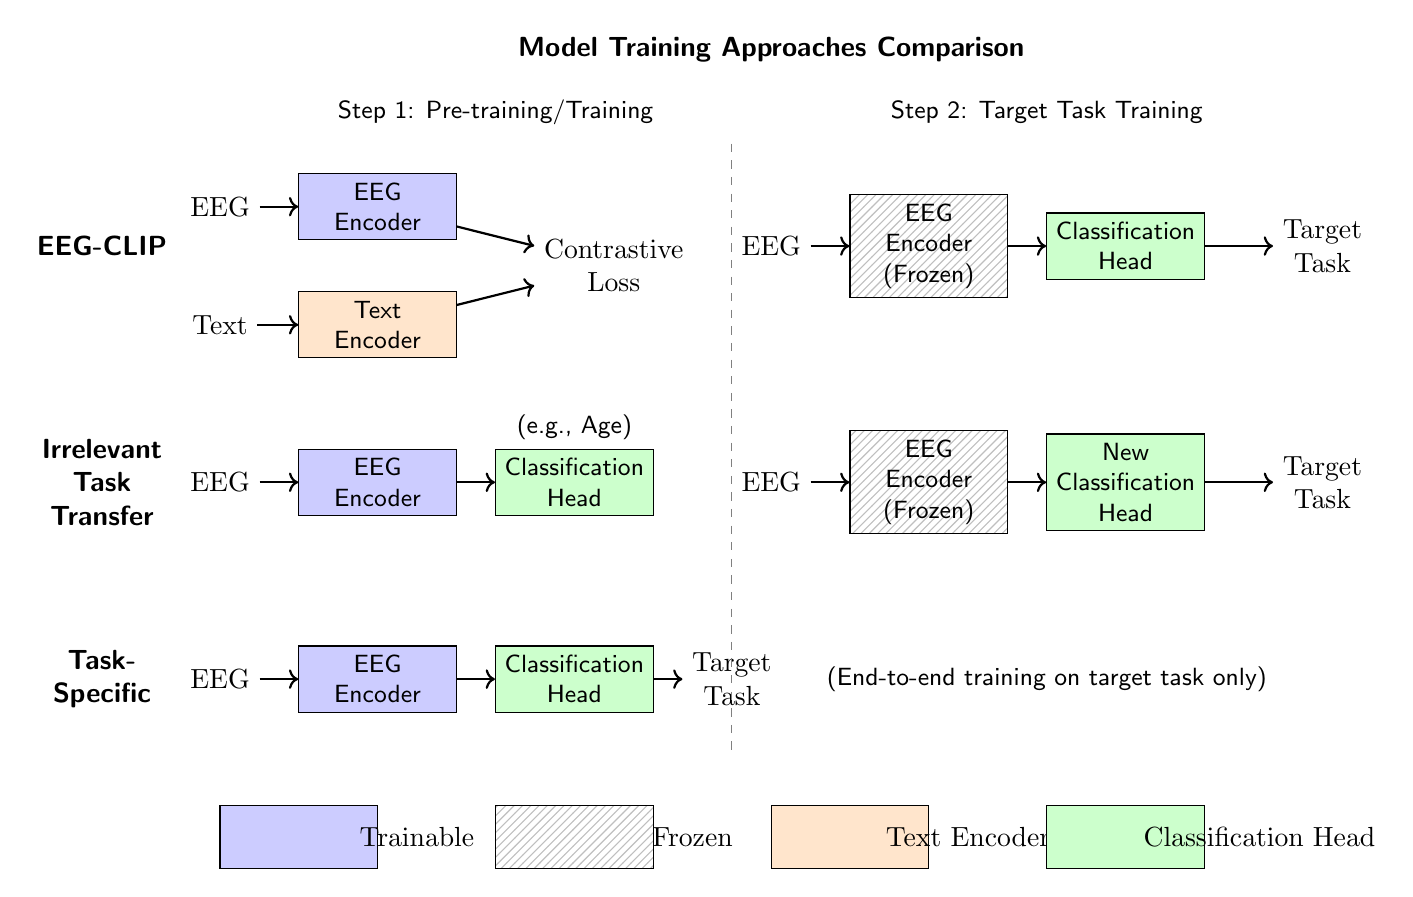
\begin{tikzpicture}[
    box/.style={rectangle, draw, minimum height=0.8cm, minimum width=2cm, font=\sffamily\small, align=center},
    encoder/.style={box, fill=blue!20},
    classifier/.style={box, fill=green!20},
    text_enc/.style={box, fill=orange!20},
    frozen/.style={box, fill=gray!30, pattern=north east lines, pattern color=gray!50},
    arrow/.style={->, thick},
    title/.style={font=\sffamily\bfseries},
    subtitle/.style={font=\sffamily\small, align=center}
]
    % Main title
    \node[title] at (7, 0) {Model Training Approaches Comparison};
    
    % Column headers
    \node[subtitle] at (3.5, -0.8) {Step 1: Pre-training/Training};
    \node[subtitle] at (10.5, -0.8) {Step 2: Target Task Training};
    
    % Method 1: EEG-CLIP
    \node[title, align=center] at (-1.5, -2.5) {EEG-CLIP};
    
    % Step 1: Contrastive pre-training
    \node[encoder] (eeg1) at (2, -2) {EEG\\Encoder};
    \node[text_enc] (text1) at (2, -3.5) {Text\\Encoder};
    \node (eeg_input1) at (0, -2) {EEG};
    \node (text_input1) at (0, -3.5) {Text};
    \draw[arrow] (eeg_input1) -- (eeg1);
    \draw[arrow] (text_input1) -- (text1);
    
    % Contrastive loss
    \node[align=center] (contrast) at (5, -2.75) {Contrastive\\Loss};
    \draw[arrow] (eeg1) -- (contrast);
    \draw[arrow] (text1) -- (contrast);
    
    % Step 2: Target task training
    \node[frozen] (eeg1_frozen) at (9, -2.5) {EEG\\Encoder\\(Frozen)};
    \node[classifier] (clf1) at (11.5, -2.5) {Classification\\Head};
    \node (eeg_input1b) at (7, -2.5) {EEG};
    \draw[arrow] (eeg_input1b) -- (eeg1_frozen);
    \draw[arrow] (eeg1_frozen) -- (clf1);
    \node[align=center] (task1) at (14, -2.5) {Target\\Task};
    \draw[arrow] (clf1) -- (task1);
    
    % Method 2: Irrelevant Task Transfer
    \node[title, align=center] at (-1.5, -5.5) {Irrelevant\\Task\\Transfer};
    
    % Step 1: Irrelevant task training
    \node[encoder] (eeg2) at (2, -5.5) {EEG\\Encoder};
    \node[classifier] (clf2a) at (4.5, -5.5) {Classification\\Head};
    \node (eeg_input2) at (0, -5.5) {EEG};
    \draw[arrow] (eeg_input2) -- (eeg2);
    \draw[arrow] (eeg2) -- (clf2a);
    \node[subtitle] (irr_task) at (4.5, -4.8) {(e.g., Age)};
    
    % Step 2: Target task training
    \node[frozen] (eeg2_frozen) at (9, -5.5) {EEG\\Encoder\\(Frozen)};
    \node[classifier] (clf2b) at (11.5, -5.5) {New\\Classification\\Head};
    \node (eeg_input2b) at (7, -5.5) {EEG};
    \draw[arrow] (eeg_input2b) -- (eeg2_frozen);
    \draw[arrow] (eeg2_frozen) -- (clf2b);
    \node[align=center] (task2) at (14, -5.5) {Target\\Task};
    \draw[arrow] (clf2b) -- (task2);
    
    % Method 3: Task-Specific
    \node[title, align=center] at (-1.5, -8) {Task-\\Specific};
    
    % Direct task training
    \node[encoder] (eeg3) at (2, -8) {EEG\\Encoder};
    \node[classifier] (clf3) at (4.5, -8) {Classification\\Head};
    \node (eeg_input3) at (0, -8) {EEG};
    \draw[arrow] (eeg_input3) -- (eeg3);
    \draw[arrow] (eeg3) -- (clf3);
    \node[align=center] (task3) at (6.5, -8) {Target\\Task};
    \draw[arrow] (clf3) -- (task3);
    
    \node[subtitle] at (10.5, -8) {(End-to-end training on target task only)};
    
    % Vertical separator
    \draw[dashed, gray] (6.5, -1.2) -- (6.5, -9);
    
    % Legend
    \node[encoder] at (1, -10) {};
    \node at (2.5, -10) {Trainable};
    \node[frozen] at (4.5, -10) {};
    \node at (6, -10) {Frozen};
    \node[text_enc] at (8, -10) {};
    \node at (9.5, -10) {Text Encoder};
    \node[classifier] at (11.5, -10) {};
    \node at (13.2, -10) {Classification Head};
    
\end{tikzpicture}
\caption{\textbf{Training approaches comparison.} Three methods for EEG classification: (1) EEG-CLIP uses contrastive pre-training with text before target task fine-tuning with frozen encoder, (2) Irrelevant Task Transfer pre-trains on an unrelated task then adapts to target task with frozen encoder, (3) Task-Specific trains directly on target task end-to-end. Components: blue = EEG encoder, orange = text encoder, green = classification head, striped = frozen/non-trainable.}
\label{fig:ssl_crosscorr}
\end{figure}

\end{document}